%!TeX root = ./../MusterAbschlussarbeit.tex

%##########################################################
% Inhalt
%##########################################################

\clearpage
\chapter{Implementierung}
\section{Umsetzung in Unity}
Der \textbf{Controller} stellt alle Funktionalitäten bereit, welche gebraucht werden, um die Lernumgebung zu initialisieren.
Er besitzt Prefabs des Agents, des GameFields und der Würfel und initialisiert diese zum Start.
Weiterhin implementiert der Controller die Funktionalität der Punktevergabe, welche für eine Mehrspielervariante genutzt werden kann.
Der Controller ist das Parent aller anderen Elemente und so ist er das zentrale Element der Steuerung. Auch das wiederholte Rollen der Würfel wird im Controller angestoßen.
Der Controller war hilfreich beim Erstellen paralleler Trainings, da dieser mehrfach in die Szene aufgenommen werden musste um mehrere Spielfelder, welche gleichzeitig bespielt werden zu initialisieren.

Der \textbf{NumberDice} implementiert die Logik, welche für das Würfeln und Visualisieren der Zahlenwürfel benötigt wird.
Die Visualisierung funktioniert mit selbst angefertigten Sprites, welche in einem sortierten Array liegen und je nach gewürfelter Zahl initialisiert und gerendert werden.
Beim wiederholten Würfeln, wird das aktuelle Sprite zerstört und ein neues initialisiert.
Damit ist gewährleistet, dass immer das aktuelle Würfelergebnis angezeigt wird.
Die Zahl des Würfels wird als Integer gespeichert, wobei er die Zahlen 1-6 annehmen kann.
Die Zahl '6' entspricht dem Zahlenjoker. \ref{fig:NumberSprites} zeigt die verwendeten Sprites für den Zahlenwürfel. 


Wie der Zahlenwürfel implementiert der \textbf{ColorDice} die Funktionalität des Würfelns der Farben.
Diese werden als String dargestellt und können folgende Werte annehmen: \{'blue', 'green','red', 'yellow', 'orange', 'joker'\}.
Zur Visualisierung wird ein Sprite erstellt, was in der gewürfelten Farbe eingefärbt wird. Ein schwarzes Feld entspricht dem gewürfelten Farbjoker.


Das \textbf{GameField} stellt das tatsächliche Spielfeld dar.
Es implementiert die benötigten Methoden um die SquareFields zu verwalten und rückzusetzen.
Außerdem wird die Anzahl der Joker in ihm gehalten. \ref{fig:Environment} zeigt neun dieser SPielfelder, welche nach Vorlage von \ref{fig:Vorlage} modelliert wurden.

Funktionalitäten:
\setlist{noitemsep}
\begin{itemize}
	\item  Visualisierung des Spielfeldes
    \item  Aktualisieren der Gruppen aller Felder
    \item  Abkreuzen der Felder
    \item  Berechnen der validen Nachbarn der Felder
    \item  Berechnen der verbleibenden Felder einer bestimmten Farbe
    \item  Rückgabe der validen Felder für die aktuell gewählten Würfel.
    \item  Reduzieren der verbleibenden Joker
    \item  Rücksetzen der Felder um ein neuest Spiel zu Starten
\end{itemize}

Die \textbf{FieldSquares} stellen die einzelnen Teilfelder des Spielfeldes dar. In Tabelle \ref{tab:Informationen in FieldSquares} wird dargestellt, welche Informationen gehalten werden.
\begin{table}[htbp]
    \centering
    \begin{tabular}{|c|c|c|}
    \hline
    \textbf{Beschreibung} & \textbf{Typ} & \textbf{Wertebereich} \\
    \hline
    Feld ist ein Sternfeld & Boolean & True / False \\
    \hline
    Farbe des Feldes & String & - \\
    \hline
    Feld ist ausgefüllt & Boolean & True / False \\
    \hline
    Feld ist verfügbar & Boolean & True / False \\
    \hline
    Clustergröße & Integer & 1-6 \\
    \hline
    X-Koordinate des Feldes & Integer & 0-14 \\
    \hline
    Y-Koordinate des Feldes & Integer & 0-6 \\
    \hline
    \end{tabular}
    \caption{Übersicht Informationen der Fieldsquares}
    \label{tab:Informationen in FieldSquares}
\end{table}

\section{Visualisierung}
Die Visualisierung des Spielfeldes erfolgt über ein angefertigtes Prefab. In diesem wurden die 105 Kästchen in einem Raster von 15x7 instanziiert und manuell mit den Informationen versehen. Dieses manuell angefertigte Spielfeld wurde als Prefab gespeichert und dient als Umgebung für den Agenten.
Zu Beginn des Spiels werden die Felder instanziiert in die Farben der hinterlegten Information in den richtigen Farben eingefärbt. Ausgefüllte Kästchen werden grau eingefärbt, diese Funktionalität wird im Fieldsquare Prefab ausgeführt. \ref{fig:Environment} zeigt den Aufbau der Trainingsumgebung. Jedes der Spielfelder besitzt einen eigenen Agenten und ist somit die Lernumgebung für genau einen Agenten. Alle Agenten trainieren gemeinsam ein Modell. Es können beliebig viele weitere Lernumgebungen hinzugefügt werden. Mehrere gleichzeitige Traingsvorgänge bedeuten jedoch wiederum einen höheren Rechenaufwand.


\section{Implementierung des Agenten}
Der Agent ist die Schnittstelle zwischen dem Environment und dem RL.
Dem Agent werden alle nötigen Informationen des Spielfeldes übergeben. Diese werden in ein neuronales Netz übertragen, welches wiederum die Ausgabewerte in einem Vektor zurück an den Agenten leitet.
Anschließend wird der Vektor verarbeitet und die gewählten Aktionen werden ausgeführt.
Für gute Aktionen erhält der Agent positive Rewards, bei schlechten Aktionen wird der Zug übersprungen. \\
Zu Beginn jeder Episode, welche einem Spielzug entspricht, muss dem Agenten der aktuelle Zustand des Feldes übermittelt werden, aus welchem er die bestmögliche Option für einen Zug berechnet. In der ML Agents Bibliothek gibt es hierfür eine vorgefertigte Methode mit dem Namen CollectObservations. Diese erzeugt einen Observationsvektor \ref{tab:Aufbau Beobachtungen}, zu welchem die Informationen der aktuellen Zustands hinzugefügt werden.
Wärend des Trainings eines Neuronalen Netzes, muss die Größe des Vektors und die Art der Werte gleich bleiben. Deswegen ist nicht möglich ein Modell auf unterschiedlichen Spielfeldern zu trainieren, da sich so die Anzahl der Beobachtungen unterscheiden würden.
\ref{lst:Code CollectObservations} erstellt anhand der Daten den Vektor aus beobachtungen und übergibt ihn an den Agenten.


Aufbau der Beobachtungen:
\begin{table}[!htbp]
    \centering
    \begin{tabular}{|c|c|c|c|}
    \hline
    \textbf{Index} & \textbf{Beschreibung} & \textbf{Type} & \textbf{Wertebereich} \\
    \hline
    0 & Anzahl der verbleibenden Joker & Float & $[0 - 1]$ \\
    \hline
    1 & Anzahl der gespielten Runden & Float & $[0 - 1]$ \\
    \hline
    2 & Ergebnis des ersten Zahlenwürfels & Float & $[0 - 1]$ \\
    \hline
    3 & Ergebnis des zweiten Zahlenwürfels & Float & $[0 - 1]$ \\
    \hline
    4-9 & Ergebnis des ersten Farbwürfels & Vector6 (Binary) & $(0, 1)^6$ \\
    \hline
    10-15 & Ergebnis des zweiten Farbwürfels & Vector6 (Binary) & $(0, 1)^6$ \\
    \hline
    16-24 & Informationen für Feld 1 & FeldVektor & - \\
    \hline
    25-33 & Informationen für Feld 2 & FeldVektor & - \\
    \hline
    ... & ... & ... & ... \\
    \hline
    953-961 & Informationen für Feld 105 & FeldVektor & - \\
    \hline
    \end{tabular}
    \caption{Zusammenfassung der Observations und Feldinformationen}
    \label{tab:Aufbau Beobachtungen}
\end{table}
    
\begin{table}[!htbp]
    \centering
    \begin{tabular}{|c|c|c|c|}
    \hline
    \textbf{Stelle im Vektor} & \textbf{Beschreibung} & \textbf{Type} & \textbf{Wertebereich} \\
    \hline
    $k*9+16$ - $k+21$ & Farbe des Feldes $k$ & Vector6 (Binary) & $(0, 1)^6$ \\
    \hline
    $k*9+22$ & Ist Feld $k$ verfügbar & Boolean & True / False \\
    \hline
    $k*9+23$ & Ist Feld $k$ abgestrichen & Boolean & True / False \\
    \hline
    $k*9+24$ & Ist Feld $k$ ein Sternfeld & Boolean & True / False \\
    \hline
    \end{tabular}
    \caption{Aufbau FeldVektor}
    \label{tab:Aufbau Feldvektor}
\end{table}

Anhand der Observations berechnet das neuronale Netz einen Ausgabevektor. Tabelle \ref{tab:Aktionbuffer} zeigt den Aufbau der hier verwendeten Beobachtungen. Mit diesem führt der Agent nun bestimmte Aktionen aus und versucht sein Ergebnis (Rewards) zu maximieren.
Anhand der gesammelten Rewards wird das neuronale Netz nun angepasst, um das bestmögliche Ergebnis zu erreichen.

\begin{table}[!h]
    \centering
    \caption{Index und Beschreibung der Variablen}
    \begin{tabular}{|c|c|c|c|}
    \hline
    \textbf{Index} & \textbf{Beschreibung} & \textbf{Typ} & \textbf{Wertebereich} \\
    \hline
    \textbf{1} & Index des gewählten ZahlenWürfels & Integer & 0-1 \\
    \hline
    \textbf{2} & Index des gewählten Farbwürfels & Integer & 0-1 \\
    \hline
    \textbf{3} & Jokerzahl & Integer & 0-4 \\
    \hline
    \textbf{4} & X-Koordinate des gewählten Feldes & Integer & 0-14 \\
    \hline
    \textbf{5} & Y-Koordinate des gewählten Feldes & Integer & 0-7 \\
    \hline
    \textbf{6} &  Action 1 für die Auswahl der Nachbarn & Continuous & - \\
    \hline
    \textbf{7} &  Action 2 für die Auswahl der Nachbarn & Continuous & - \\
    \hline
    \textbf{8} &  Action 3 für die Auswahl der Nachbarn & Continuous & - \\
    \hline
    \textbf{9} &  Action 4 für die Auswahl der Nachbarn & Continuous & - \\
    \hline
    \end{tabular}
    \label{tab:Aktionbuffer}
\end{table}

Das Vergeben von Rewards lehnt sich an die Punktevergabe im Spiel wie nach Vorlage \ref{fig:Vorlage} an. Der Agent erhält Belohnungen, wenn er auch Punkte im gespielten Spiel erlangen würde. In \ref{tab:rewards} ist eine Übersicht der Belohnungen. Aus dieser lässt sich ablesen, welche Aktion welchen Reward auslöst.

\begin{table}[htbp]
    \centering
    \begin{tabular}{|c|c|}
    \hline
    \textbf{Aktion} & \textbf{Erhaltene Belohnung} \\
    \hline
    Abkreuzen eines Sternfeldes & 2 \\
    Ausfüllen einer kompletten Spalte & 1-5 abhängig der Spalte\\
    Ausfüllen einer kompletten Farbe & 5 \\
    Verbleibende Joker zum Ende des Spiels & 1 / verbleibendem Joker \\
    \hline
    \end{tabular}
    \caption{Belohnungen für bestimmte Aktionen}
    \label{tab:rewards}
\end{table}



\newpage
\section{Spezifikation des Alghorithmus}
Im folgenden wird der Ablauf zum Wählen der Felder erläutert. Im Beispiel wird der Ausgabevektor \textbf{(1 , 1 , 0 , 3 , 4 , 0.6 , 0.5 , 0.4 , 0.8)} verwendet. \\
Die ersten beiden Stellen des Ausgabevektors entsprechen den gewählten Würfeln.
Im ersten Schritt werden alle Felder des Spielfelds untersucht, ob sie ein valides Ziel für das gewürfelte Ergebnis bilden. Dies ergibt sich aus der Gruppe der Spielfelder, der Farbe und ob das Kästchen verfügbar ist.
Valide Felder werden in eine Liste (availableFields) aus Verfügbaren Feldern geschrieben. Abb. \ref{fig:alg1} zeigt den beschriebenen Zustand des Feldes.\\
Abb. \ref{fig:alg2} bildet den nächsten Schritt im Algorhitmus ab.
Es wird geprüft, ob die gewählten Koordinaten in availableFields vorhanden sind.
Wenn kein Feld verfügbar ist, wird die Episode abgebrochen und der Agent überspringt seinen Zug.
Sofern der Agent ein valides Feld gewählt hat, wird dieses in eine weitere Liste (pickedFields) geschrieben und benachbarte Felder der selben Gruppe werden zurückgegeben. \\
Im nächsten Schritt wird jedem der verfügbaren Nachbarn abhängig der Gesamtanzahl ein Wertebereich zwischen 0 und 1 zugewiesen, dies wird in \ref{fig:alg3} und \ref{tab:field_ranges} verdeutlicht. Anhand des diskreten Wertes des Ausgabevektors wird das zugehörige Feld in eine Liste aus den gewählten Feldern geschrieben.
\begin{table}[!h]
    \centering
    \begin{tabular}{|c|c|c|}
    \hline
    \textbf{FeldKoordinaten} & \textbf{von} & \textbf{bis} \\
    \hline
    (3,5) & 0 & 0.33 \\
    \hline
    (4,4) & 0.33 & 0.66 \\
    \hline
    (3,3) & 0.66 & 0.99 \\
    \hline
    \end{tabular}
    \caption{Bereiche für bestimmte Felder}
    \label{tab:field_ranges}
\end{table}

Für alle gewählten Felder werden die benachbarten Felder zurückgegeben und der vorherige Schritt wiederholt.
Wenn so viele Felder gewählt, wie erwürfelt wurden, werden die Felder anschließend ausgefüllt und auf Rewards überprüft.Die wird in Abbildung \ref{fig:alg4} dargestellt.

\begin{figure}[!h]
	\centering
	\includegraphics[width=0.45\textwidth]{Bilder/Erklärung_Alghorhitmus_1.png}
	\caption{Valide Felder für das gewählte Würfelergebnis wurden markiert}
    \label{fig:alg1}
\end{figure}

\begin{figure}[!h]
	\centering
	\includegraphics[width=0.45\textwidth]{Bilder/Erklärung_Alghorhitmus_2.png}
	\caption{Feld(3,4) wird in die pickedField Liste aufgenommen und benachbarte Felder werden zurückgegeben.}
    \label{fig:alg2}
\end{figure}


\begin{figure}[!h]
	\centering
	\includegraphics[width=0.45\textwidth]{Bilder/Erklärung_Alghorhitmus_3.png}
	\caption{Feld(4,4) ist das nächste gewählte Feld und wird in pickedFields aufgenommen}
    \label{fig:alg3}
\end{figure}


\begin{figure}[!h]
	\centering
	\includegraphics[width=0.45\textwidth]{Bilder/Erklärung_Alghorhitmus_4.png}
	\caption{Felder wurden gewählt und ausgefüllt}
    \label{fig:alg4}
\end{figure}
\clearpage
\section{Auswertung der erreichten Punkte}
Um die verschiedenen Modelle bewerten zu können, wurden die erreichten Punkte aufgezeichnet und anschließend ausgewertet.
Im Verlauf eines Spiels werden alle erreichten Punkte im Spielfeld gespeichert. 
Nach 30 gespielten Zügen wird die erreichte Punktzahl in eine Logdatei geschrieben.
In \ref{fig:punktWolke} lässt sich ableiten, dass Belohnungen nur dann verteilt werden, wenn es auch zu einer Punktewertung kommt. Die beiden Werte sind lediglich um 30 Punkte verschoben, da der Spieler das Spiel mit -30 Punkten beginnt.

\begin{figure}[!h]
	\centering
	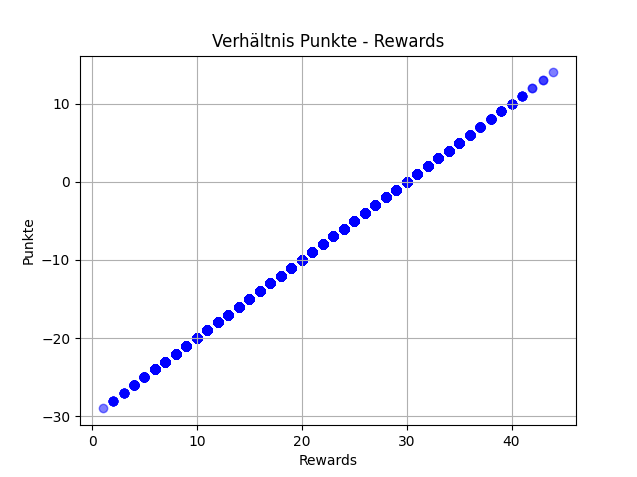
\includegraphics[width=0.45\textwidth]{Bilder/punktWolke.png}
	\caption{Verhältnis Rewards zu Punkten}
    \label{fig:punktWolke}
\end{figure}


Die Logdateien wurden anschließend mit Python ausgewertet. In \ref{lst:ImportLogfiles} werden die angegebenen Punkteaufzeichnugnen importiert und jedem Datensatz einen Titel zur Beschriftung der Graphen hinzugefügt. Im Anschluss wird hier der gleitende Durchschnitt abhängig der gewählten Anzahl an Spielen berechnet. 

Dabei werden erst alle Werte addiert und der Mittelwert gebildet.Danach wird der herrausrotierende Wert abgezogen und um den Neuen ergänzt. Auf diese Weise muss jeder Wert lediglich 2 mal gelesen werden. \\ In der Methode \ref{lst:DisplayGraph} können nun variabel Graphen gewählt und anschließend gerendert werden. Vor Methodenaufruf, muss die Liste an anzuzeigenden Graphen bearbeitet werden und in den Methodenaufruf übergeben werden. 



